%% Appendix tex file by Meldonization.

\chapter{文内常用约定} \label{apdx:nomenclature}
\section{物理符号含义} \label{apdx:symbol}
\begin{multicols}{2}
\begin{tabularx}{1.0\linewidth}{@{\extracolsep{\fill}}lr}
\centering
$a$      	     			&     轨道半长径 		\\
$d$      	     			&     质点二体间距离	 	\\
$P$      	     			&     轨道周期	 		\\
$e$      	     			&     轨道偏心率 		\\
$i$          	     			&     轨道倾角 			\\
%$\omega$      			&     近心点角距 		\\
%$\Omega$     			&     升交点经度 		\\
%$f$              			&     真近点角   			\\
$\tif{M}_\odot$          		&     太阳质量   			\\
$M_\tif{s}$          		&     恒星质量   			\\
$\tif{R}_\odot$          		&     太阳半径   			\\
$R_\tif{s}$          		&     恒星半径   			\\
$\tif{M}_\tif{J}$          		&     木星质量   			\\
$\tif{M}_\oplus$          	&     地球质量   			\\
$M_\tif{p}$         	 	&     行星质量   			\\
$m$         	 			&     视星等   			\\

\end{tabularx}
\columnbreak



\end{multicols}

\newpage


\section{首字母缩写}  \label{apdx:acronym}
本文首字母缩写主要参考自书籍\citen{AstroDict},按照字母先后顺序排列如下:
\begin{multicols}{2}
\begin{tabularx}{1.0\linewidth}{@{\extracolsep{\fill}}lr}
\centering
AST3           &   南极巡天望远镜     	   	  \\  
CCD		   &   电荷耦合器件			   \\
CSTAR        &   南极之星望远镜阵列 		   \\  
FFP             &   自由飘游行星        		   \\ 
FOV            &   视场			     		   \\ 
GB              &   银核球				   \\
GD              &   银盘				  	    \\
GI                &   引力不稳定              		    \\
IAU             &    国际天文学联合会   	    	    \\
MMR           &   平运动共振   	                     \\   
MMSN         &   最小质量原行星盘                 \\
NIAOT         &   南京天文光学技术研究所       \\
OGLE         &    光学引力透镜实验   	     	     \\
PPD            &    原行星盘   	   	     	     \\
RV              &    视向速度                    	     \\
TNO           &    海外天体                    	     \\
TTV            &    凌星计时变化             	     \\
YSO           &    初期恒星体                	     \\

\end{tabularx}
\columnbreak



\end{multicols}




\chapter{二体运动示意图} \label{apdx:twobodyproblem}

\begin{figure}[h]
\centering
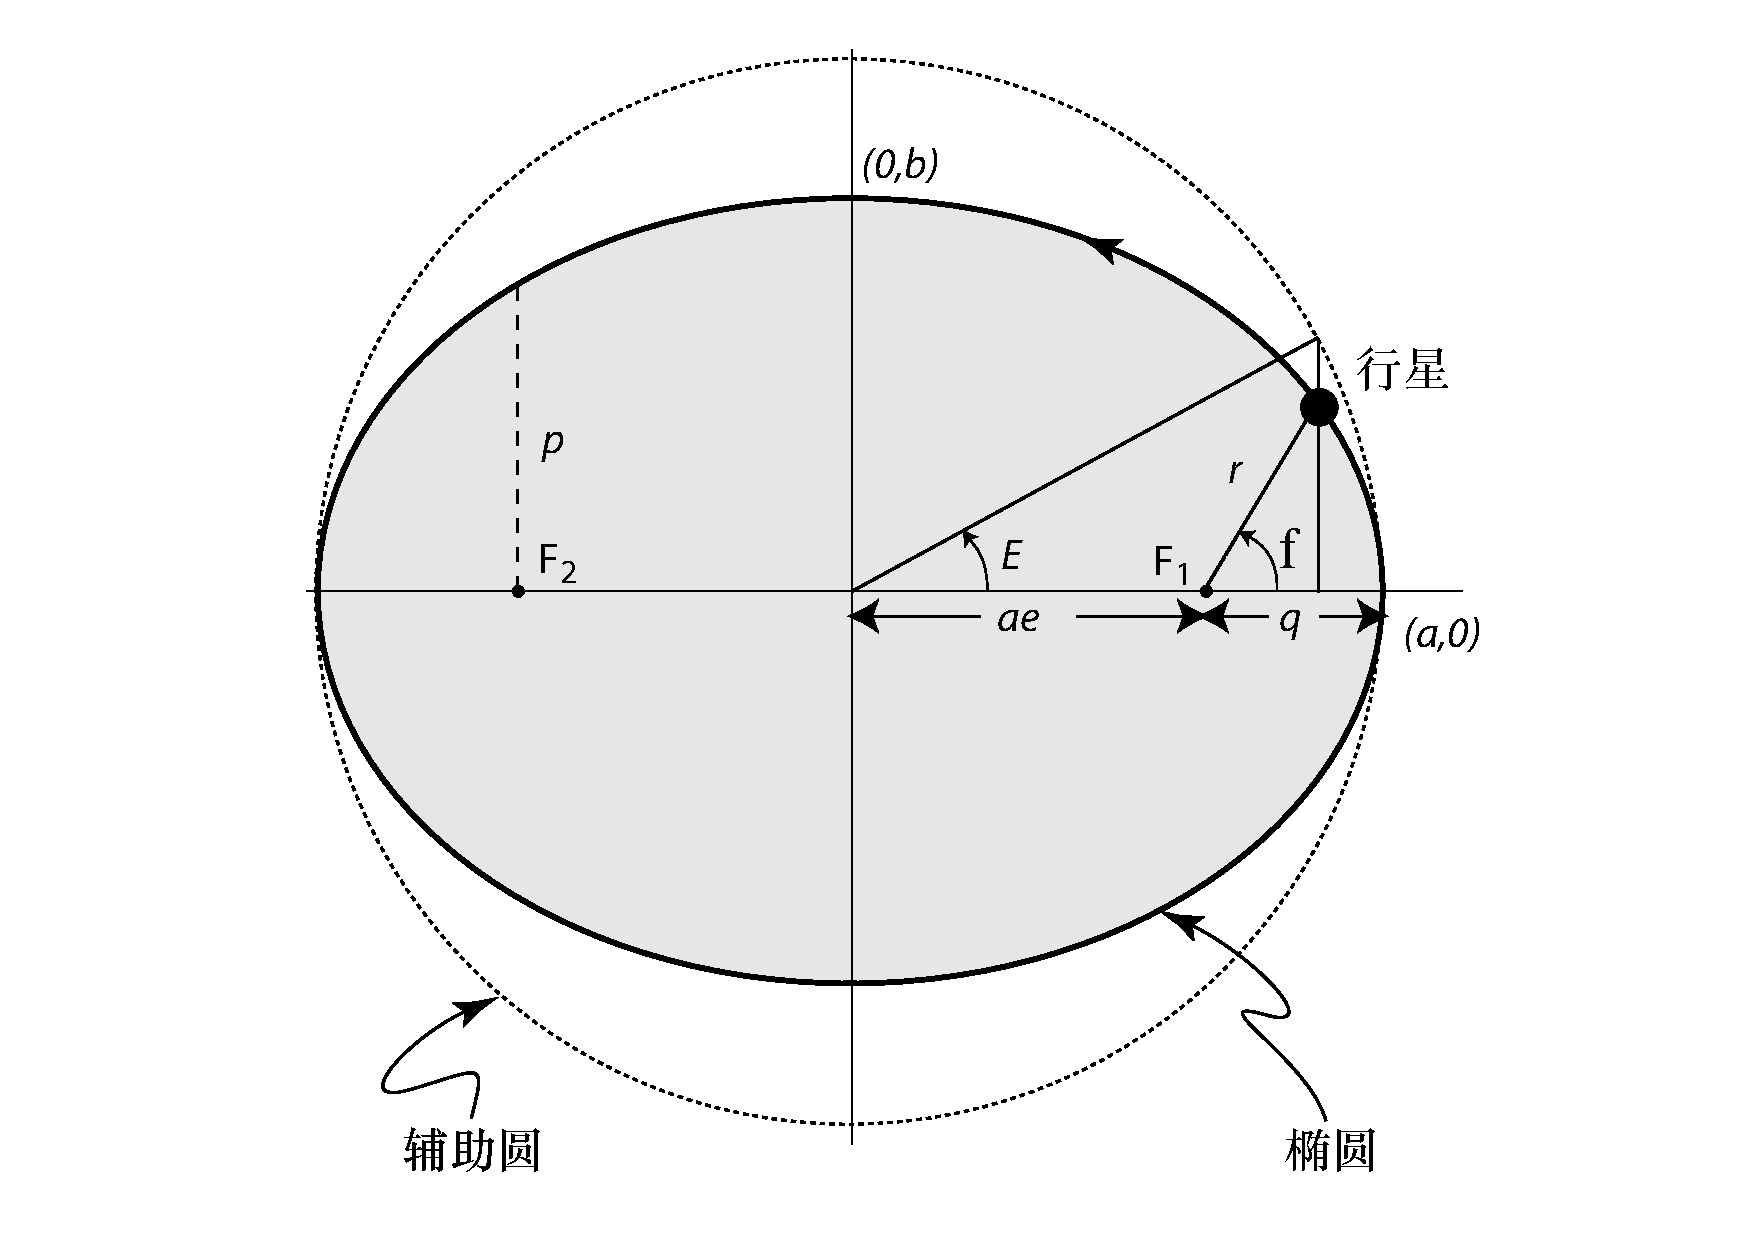
\includegraphics[width=0.95\textwidth]{figures/appendix/f1_ellipse.pdf}
\caption{二体在轨道平面内的椭圆运动示意图,图片来源 Perryman。}
\label{fig:ellipse}
\end{figure}

在次方反比的中心引力作用下,二体的运动轨迹为封闭的圆锥曲线\cite{Newton1687}。
图\ref{fig:ellipse} 和 \ref{fig:3dorbit} 展示的是椭圆二体运动示意图,其中 $a,\,e,\,i,\,\omega,\,\Omega,\,f$ 
被称作描述椭圆二体运动的六个轨道常数,文内符号几乎均沿袭自书本\citen{MurrayDermott1999ssd}。
在中心天体坐标系中,行星距离主星的标量距离 $r$ 可表示为:
\begin{equation} \label{radialdistance}
r = \frac{a(1-e^2)}{1+e\cos f}
\end{equation} %\myequation{二体运动的径向距离与轨道根素的关系}

\begin{figure}[t]
\centering
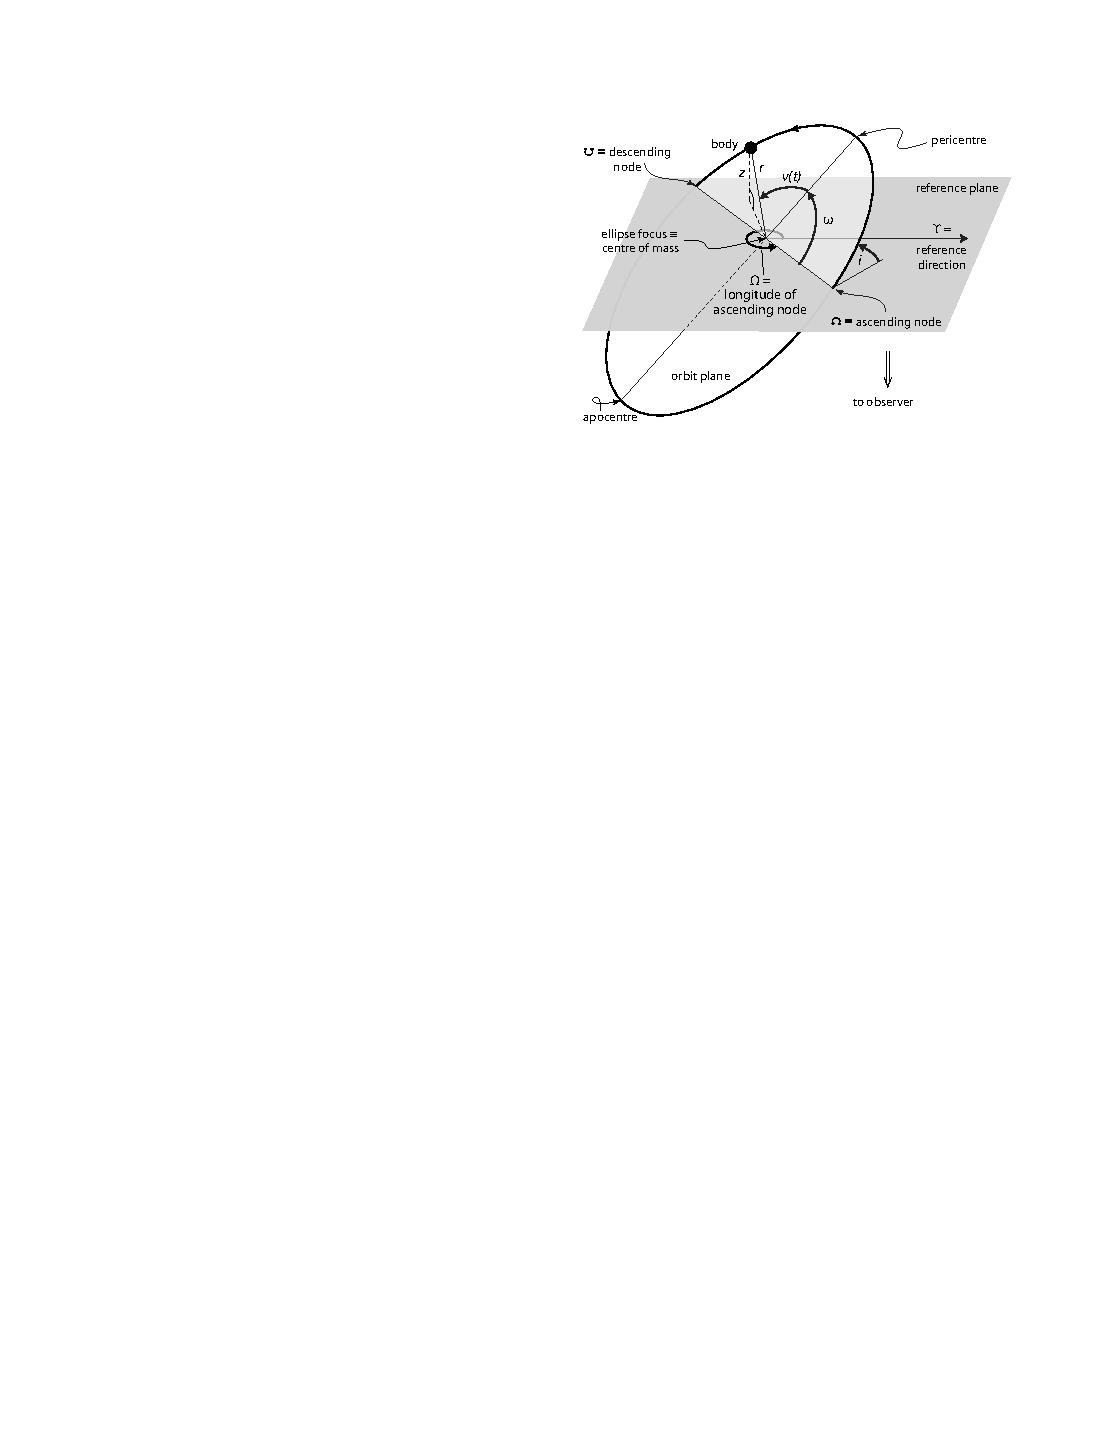
\includegraphics[width=0.95\textwidth]{figures/appendix/f2_3dorbit.pdf}
\caption{椭圆二体运动轨道在三维空间内的示意图,图内标识分别为轨道根数与参考系。图片来源 Perryman。}
\label{fig:3dorbit}
\end{figure}



